\begin{figure}[H]
    \centering
    \definecolor{surfaceblue}{RGB}{75,145,205}
    \definecolor{gradientred}{RGB}{185,45,45}
    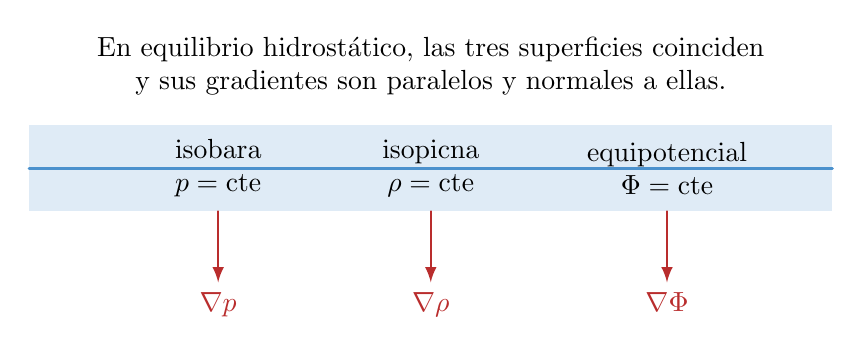
\begin{tikzpicture}[x=1cm,y=1cm,line cap=round,line join=round]
        \fill[surfaceblue!18] (0.6,1.15) rectangle (10.8,2.25);
        \draw[surfaceblue,line width=1.1pt] (0.6,1.70) -- (10.8,1.70);

        \node[align=center] at (3.0,1.70)
            {isobara\\$p=\mathrm{cte}$};
        \node[align=center] at (5.7,1.70)
            {isopicna\\$\rho=\mathrm{cte}$};
        \node[align=center] at (8.7,1.70)
            {equipotencial\\$\Phi=\mathrm{cte}$};

        \draw[gradientred,-latex,line width=0.9pt]
            (3.0,1.15) -- (3.0,0.25);
        \node[gradientred,below] at (3.0,0.25) {$\nabla p$};

        \draw[gradientred,-latex,line width=0.9pt]
            (5.7,1.15) -- (5.7,0.25);
        \node[gradientred,below] at (5.7,0.25) {$\nabla\rho$};

        \draw[gradientred,-latex,line width=0.9pt]
            (8.7,1.15) -- (8.7,0.25);
        \node[gradientred,below] at (8.7,0.25) {$\nabla\Phi$};

        \node[align=center] at (5.7,3.00)
            {En equilibrio hidrostático, las tres superficies coinciden\\
             y sus gradientes son paralelos y normales a ellas.};
    \end{tikzpicture}
    \caption{Relación geométrica entre superficies isobaras, isopicnas y equipotenciales.}
\end{figure}